
\section{Synchronous Monitoring}

%-------------------------------------------------------------------------


\iffalse
\begin{frame}{Synchronous Monitoring}


An \LTLtri monitor can evaluate an \LTL formula $\varphi$ in a centralized 
setting where each proposition represents the global state of the system. We 
show in Section \ref{sec:DSM} and Chapter \ref{chap:DAM} that in a framework of several synchronous or asynchronous 
{\em unreliable} monitors, naive local monitoring may lead to inconsistent 
global verdicts for $\varphi$. 

\note{ we propose a framework for synchronous distributed 
fault-tolerant runtime verification (RV). To this end, we make a link between 
RV and consensus in a failure-prone distributed environment by 
proposing an automata-based algorithm.
}

\end{frame}

\fi


\begin{frame}{Synchronous Monitoring}

\begin{block}{Distributed Synchronous Setting}
Finite trace $\alpha = s_0 s_1 \cdots s_k$ ;\\
Set of synchronous monitors $\monitor =\{M_1, M_2, \cdots , M_n\}$ ;\\
Correctness property expressed by an \LTL formula $\varphi$.

\note{1. In the decentralized synchronous setting, we assume the system under scrutiny 
generates a finite trace $\alpha = s_0 s_1 \cdots s_k$ and is inspected by a set 
of synchronous monitors $\monitor =\{M_1, M_2, \cdots , M_n\}$ with respect to 
a correctness property expressed by an \LTL formula $\varphi$. The monitors 
communicate with each other by sending and receiving messages in 
{\em synchronous rounds}, and through point-to-point bidirectional reliable 
communication links. The decentralized crash-resilient synchronous monitoring 
can be reduced to the uniform consensus problem in the crash failure 
model.\\ }

\end{block}

\begin{block}{Algorithm Sketch}
\begin{enumerate} 

\item takes a \Def{sample} from state $s_j$;

\note{\Def{2-reads} the value of a subset of propositions in $s_j$, which may 
result in a {\em partial} observation of $s_j$.\\}

\item \Def{broadcasts} a message containing its current observation, and \Def{receives} messages from other monitors;

\note{\Def{3-at every} synchronous round, {\em broadcasts} a message containing its 
current observation of the underlying system, and then waits for messages from 
other monitors.\\}

\item performs a \Def{local computation} and updates its current observation;

\note{\Def{4-based on the messages received} at each round, executes a local 
computation, updates its current observation by incorporating observations of 
other monitors, and composing the message to be sent at next round.\\}

\item \Def{emits} a truth value from $\mathbb{B}_3$.

\note{\Def{5-finally evaluates} $\varphi$ at the end of communication rounds and 
subsequently emits a truth value from $\mathbb{B}_3$. }

\end{enumerate}

\end{block}

\end{frame}




\begin{frame}{Synchronous Monitoring}

\begin{block}{Uniform Consensus}
Eeach process proposes a value, and the processes have to collectively agree on the same value. 


\begin{itemize}
\item {\bf Validity:} \ A decided value is a proposed value.

\item {\bf Agreement:} \ No two processes decide different values.

\item {\bf Termination:} \ Every correct process decides.
\end{itemize}
\end{block}

\begin{block}{Validity Specification in Synchronous Monitoring}

The decided value must be the same value that a centralized monitor with full 
view of the system would compute.

\end{block}

\begin{block}{Number of Rounds}
The lower bound on the number of rounds required to consistently monitor the system is $f+1$, where $f$ is the total number of crashes the system can tolerate.

\note{It is easy to see that our decentralized synchronous monitoring problem, 
described in Section~\ref{sec:PS}, is similar to the uniform consesus problem that was described in Section \ref{sec:introDSM}. It is also straightforward to verify that the lower bound on the number of rounds required to consistently monitor the system is $f+1$, where $f$ is the total number of crashes the system can tolerate. The proof would be similar to 
the proof of the lower bound on the number of rounds required for the consensus 
algorithm that copes with $f$ process crashes.

}



\end{block}



\note{In the consensus problem, each process proposes a value, and the processes 
have to collectively agree on the same value. Of course, a process can crash 
before deciding a value. Moreover, in order to be meaningful, the value that is 
decided has to be related to the values that are proposed. This is captured by 
the following specification.}





\note{
The validity and agreement properties define the safety property of the 
consensus problem. Validity relates the output to the inputs, while agreement 
captures the difficulty of the problem. Termination is the liveness property of 
the consensus problem. It states that at least the processes that do not crash 
have to decide. In a synchronous setting and in the presence of faults, 
consensus is solvable in $f+1$ rounds, where $f$ is the maximum number of 
processes than can crash.

In the synchronous monitoring problem, the validity specification is that the 
decided value must be the same value that a centralized monitor that has full 
view of the system would compute.
}







\end{frame}




\begin{frame}{Synchronous Monitoring}

\begin{block}{Local Monitor Algorithm}

\begin{figure}
 \centering
 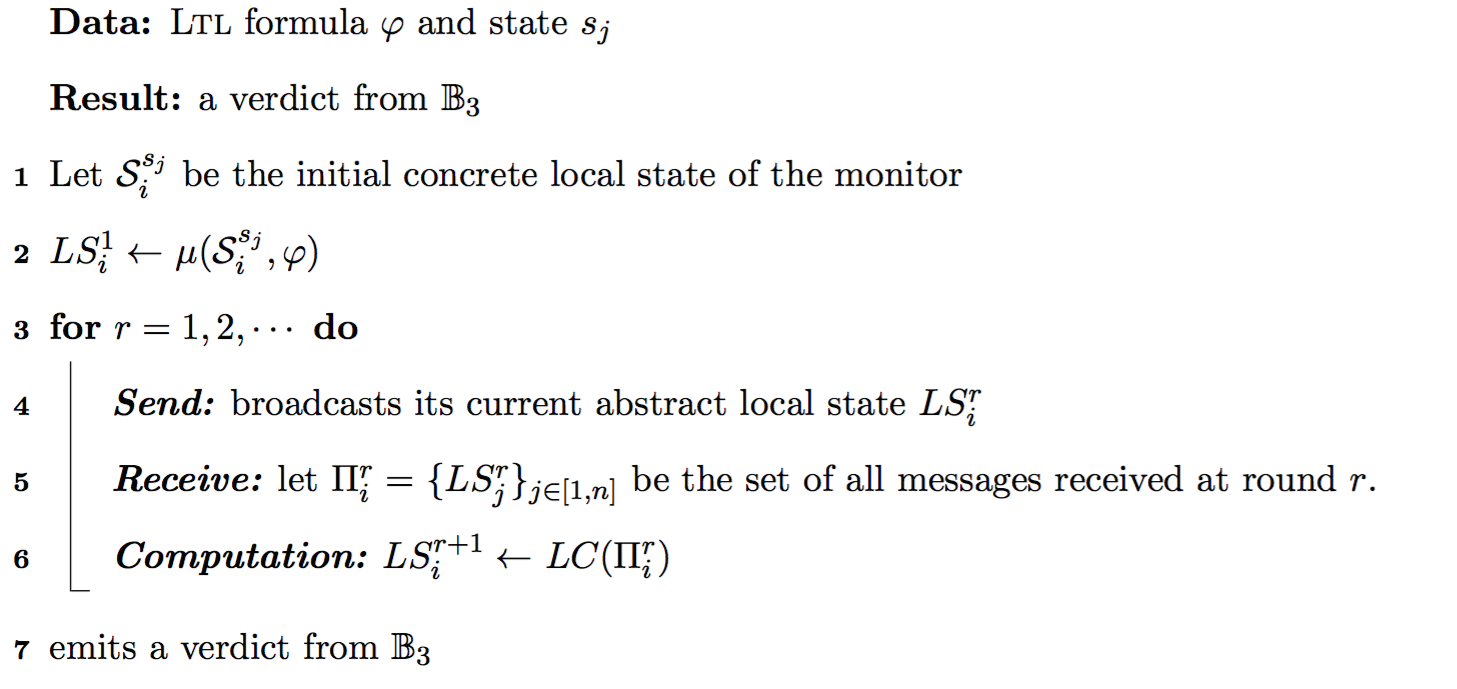
\includegraphics[scale=.3, angle=-360]{figures/synchalgo}
 \end{figure}

\end{block}

\end{frame}



\begin{frame}{Challenges in Synchronous Monitoring}


\begin{example}
Let $\varphi = \F (a \, \wedge \, b)$, $\AP=\{a, b\}$, and $\monitor =\{M_1, 
M_2, M_3, M_4\}$. Suppose $s=\{a,b\}$ is the current global state of the 
system, and the initial samples of the monitors are as follows:\\


\begin{center}

\begin{tabular}{| c |c |c|}

\multicolumn{3}{c}{sample} \\
\hline
&$a$&$b$\\
\hline
$M_1$ & $\tru$  & $\natural$\\
$M_2$ & $\natural$ & $\tru$\\
$M_3$ & $\natural$ & $\tru$ \\
$M_4$ & $\natural$ & $\tru$ \\
%$M_5$ & $\natural$ & $true$ \\
\hline
\end{tabular}
\quad
\begin{tabular}{| c |c |c|}
\multicolumn{3}{c}{round 1} \\
\hline
&$a$&$b$\\
\hline
$M_1$ & crashed & crashed\\
$M_2$ & $\tru$ & $\tru$\\
$M_3$ & $\natural$ & $\tru$ \\
$M_4$ & $\natural$ & $\tru$ \\
%$M_5$ & $\natural$ & $true$ \\
\hline
\end{tabular}


\end{center}


\begin{center}
\begin{tabular}{|c |c |c|}
\multicolumn{3}{c}{round 2} \\
\hline
&$a$&$b$\\
\hline
$M_1$ & crashed & crashed\\
$M_2$ & crashed & crashed\\
$M_3$ & $\tru$ & $\tru$ \\
$M_4$ & $\natural$ & $\tru$ \\
%$M_5$ & $\natural$ & $true$ \\
\hline
\end{tabular}
\quad
\begin{tabular}{| c |c |c|}
\multicolumn{3}{c}{round 3} \\
\hline
&$a$&$b$\\
\hline
$M_1$ & crashed & crashed\\
$M_2$ & crashed & crashed\\
$M_3$ & $\tru$ & $\tru$  \\
$M_4$ & $\tru$ & $\tru$  \\
%$M_5$ & $true$ & $true$  \\
\hline
\end{tabular}   

\end{center}

\end{example}
 
\end{frame}


\begin{frame}{Synchronous Monitoring}
\begin{block}{Challenge}

If each monitor broadcasts its sample ~$\Rightarrow$ ~ the message size is \Def{$|\AP|$}

\end{block}


\begin{block}{Reducing the Message Size Overhead}
We introduce an algorithm which decreases the message size from $|\AP|$ to  \Def{$\log(m_\monstate)$} where $m_\monstate$ is the number of outgoing transitions from monitor state $\monstate$.

\end{block}





\note{One can see in the above example, in case each monitor broadcasts its concrete 
local state, namely, if the abstract local state is the same as the concrete 
local state, then each message sent by a monitor is a register that consists of 
$|\AP|$ elements, one for each atomic proposition in $\AP$. Our goal is to 
decrease the message size overhead, hence we introduce an algorithm that 
decreases the message size from $|\AP|$ bits to something 
significantly lower. In Section \ref{sec:SAM}, we introduce an algorithm which 
decreases the message size overhead in synchronous distributed monitoring. The 
algorithm solves the synchronous distributed monitoring problem in $f +1$ 
rounds of communication with message size of $\log(m_\monstate)$, where $m_\monstate$ is the number of outgoing transitions from monitor state $\monstate$ in an \Exltl~that will be introduced in Section \ref{sec:SAMExltl}.
}



\end{frame}


\begin{frame}{Automata-based Synchronous Monitoring}

\begin{block}{The General Idea}

\begin{itemize}

\item Each local monitor $M_i$ evaluates the input formula and computes a \Def{possible} set of verdicts;

$$\verdict_i = \{\delta(\monstate, s') \mid s' \in 
\pevent(\sample_i^s)\}$$ \\


\note{Each \Def{possible verdict} is a monitor state that can be reached by a possible global state from viewpoint of monitor $M_i$.}


\item At each round, each monitor $M_i$ broadcasts its verdict set $V_i$, and computes a new verdict set by applying the \Def{intersection} function on the verdict sets received from other monitors;

$$\verdict_i^{r+1} = LC(\Pi_i^r) = \bigcap_{j \in [1, n]} \{ \verdict_j^r\} = 
\bigcap_{j \in [1, n]} \{\verdict_j^r\}$$


\item After $f+1$ rounds of communication, each monitor emits the verdict that a centralized monitor that has the global view of the system would compute.


\end{itemize}

\end{block}

\end{frame}



\begin{frame}{Automata-based Synchronous Monitoring}

\begin{block}{Local Monitor Algorithm}

\begin{figure}
 \centering
 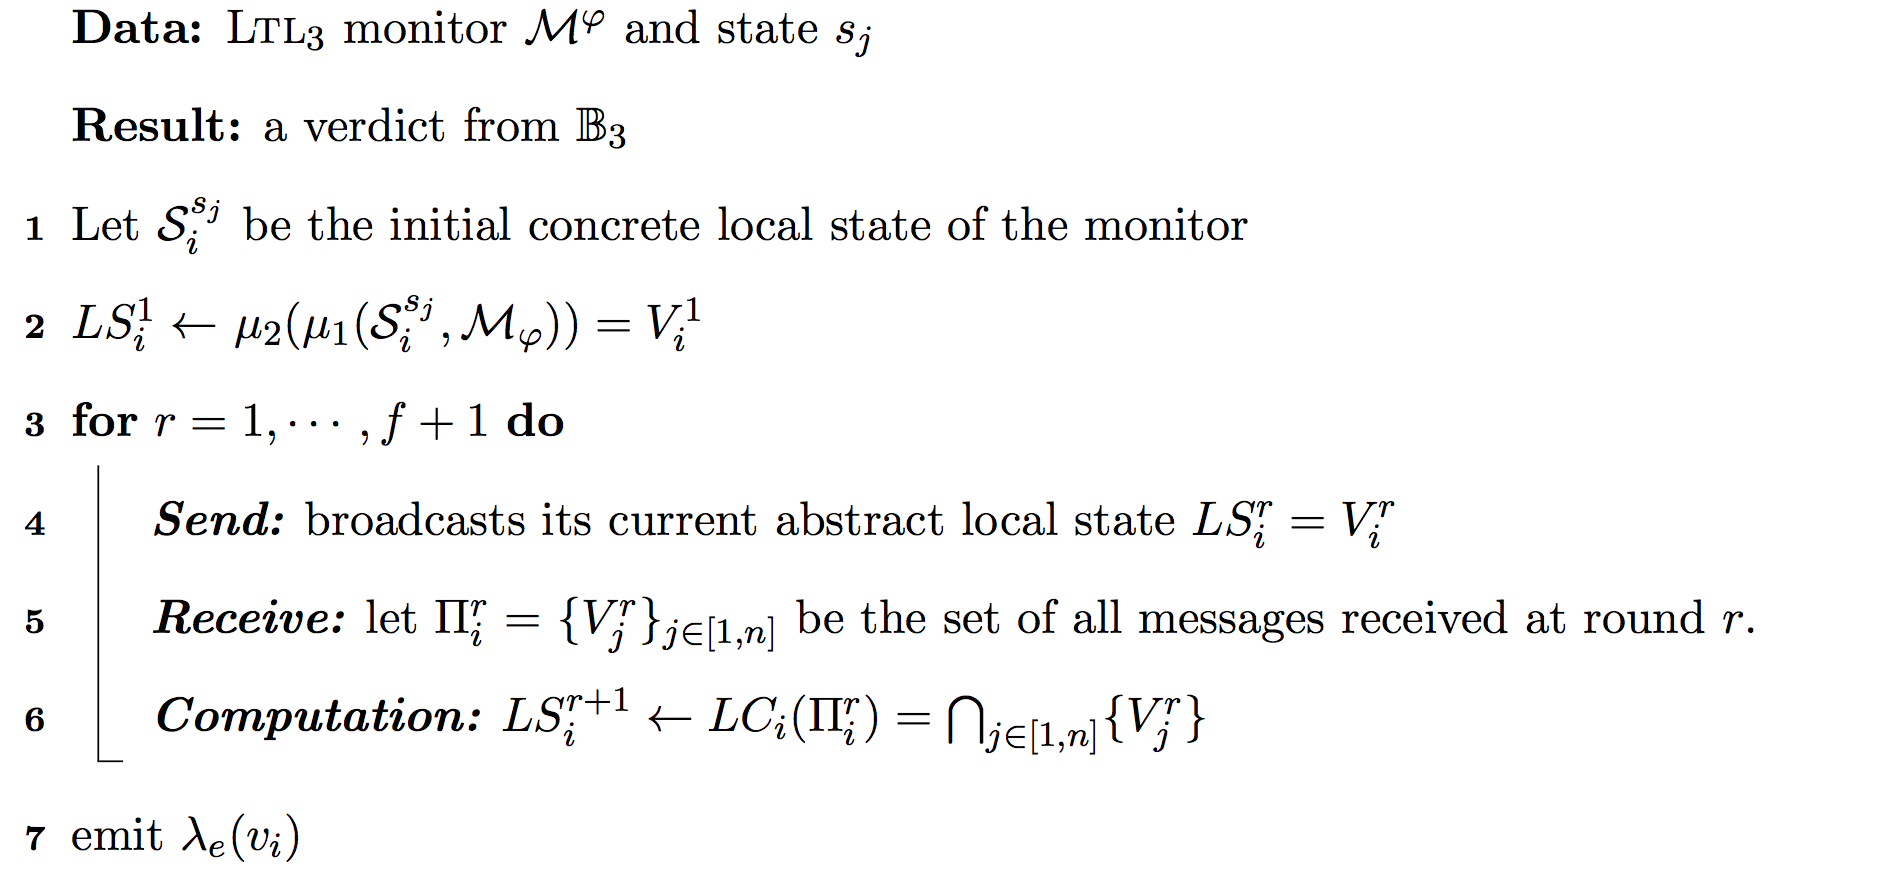
\includegraphics[scale=.3, angle=-360]{figures/localmonalgo2}
 \end{figure}

\end{block}

\end{frame}





\begin{frame}{Automata-based Synchronous Monitoring}

\begin{example}

Let $\varphi = \F (a \wedge b)$.

\begin{figure}[H]
\centering
\begin{tikzpicture}[->,>=stealth',shorten >=1pt,auto,node distance=4.8cm,
                    semithick, initial text={}, initial where=right]
  \tikzstyle{every state}=[scale=0.65, every node/.style={scale=0.65}]

  \node[initial,state] (A)                {$\monstate_0$};
  \node[state, accepting]         (B) [left of  = A] {$\monstate_\top$};

  \path (A) edge              node {$ \{a,b\}$} (B)
 
            edge [loop above] node {$\{a\}, \{b\}, \emptyset$} (A) ;
        
\end{tikzpicture}    
\caption{\LTLtri monitor of $\varphi = \F(a \wedge b)$.}
\end{figure}

And suppose the initial samples of the monitors are as follows:

\begin{center}

\begin{tabular}{| c |c |c |c|}
\multicolumn{3}{c}{sample} \\
\hline
&$a$&$b$&$\verdict_i^1$\\
\hline
$M_1$ & $\tru$  & $\natural$ & $\{\monstate_0, \monstate_\top\}$\\
$M_2$ & $\natural$ & $\tru$ &  $\{\monstate_0, \monstate_\top\}$\\
$M_3$ & $\natural$ & $\natural$ &  $\{\monstate_0, \monstate_\top\}$ \\
$M_4$ & $\natural$ & $\natural$ &  $\{\monstate_0, \monstate_\top\}$\\
%$M_5$ & $\natural$ & $true$ \\
\hline
\end{tabular} 

\end{center}

\end{example}

\end{frame}




\begin{frame}{Automata-based Synchronous Monitoring}

\begin{example}

\begin{center}
\begin{tabular}{| c |c|}
\multicolumn{2}{c}{round 1} \\
\hline
&$\verdict_i^2$\\
\hline
$M_1$ & crashed\\
$M_2$ & $\{\monstate_0, \monstate_\top\}$\\
$M_3$ & $\{\monstate_0, \monstate_\top\}$ \\
$M_4$ & $\{\monstate_0, \monstate_\top\}$ \\
%$M_5$ & $\natural$ & $true$ \\
\hline
\end{tabular}
\quad
\begin{tabular}{| c |c|}
\multicolumn{2}{c}{round 2} \\
\hline
&$\verdict_i^3$\\
\hline
$M_1$ & crashed\\
$M_2$ & crashed\\
$M_3$ & $\{\monstate_0, \monstate_\top\}$ \\
$M_4$ & $\{\monstate_0, \monstate_\top\}$ \\
%$M_5$ & $\natural$ & $true$ \\
\hline
\end{tabular}
\quad
\begin{tabular}{| c |c|}
\multicolumn{2}{c}{round 3} \\
\hline
&$\verdict_i^4$\\
\hline
$M_1$ & crashed\\
$M_2$ & crashed\\
$M_3$ & $\{\monstate_0, \monstate_\top\}$ \\
$M_4$ & $\{\monstate_0, \monstate_\top\}$ \\
%$M_5$ & $\natural$ & $true$ \\
\hline
\end{tabular} 
\end{center}

As we see $|\verdict_3|=|\verdict_4| > 1$. Therefore, they cannot emit the correct verdict $\top$  as  we have $[\{a, b\} \models_3 \F(a \wedge b)] = \top$.
\end{example}

\begin{block}{Insufficiency of \LTLtri Monitor}
The \LTLtri monitor of $\varphi = \F (a \wedge b)$ is not sufficient to distinguish 
the correct verdict when local monitors have partial view of the system.


\note{As we observe, at the end of round $3$ (namely, $f+1$), the local monitors still 
cannot decide a single verdict since $|\abstate_i^4| > 1$. This is because the 
\LTLtri monitor of $\varphi = \F (a \wedge b)$ is not sufficient to distinguish 
the correct verdict when local monitors have partial view of the system. In 
particular, monitors $M_3$ and $M_4$ both have $\{\monstate_0, 
\monstate_\top\}$ as their verdicts, while $[\{a, b\} \models_3 \F(a 
\wedge b)] = \top$. That is, the monitors cannot map their collective verdicts 
to the verdict of a monitor that has the global view of the system. 


In order to resolve this insufficiency, we introduce an algorithm that 
constructs an `\Exltl'. The algorithm receives as input an \LTLtri monitor and 
solely based on the structure of the input monitor, it determines whether to add 
new monitor states to the original \LTLtri monitor. The \Exltl~then is used in 
each local monitor $M_i$'s algorithm (Algorithm \ref{alg:localmonalgo2}) to 
consistently solve the decentralized synchronous monitoring problem. As 
described earlier, the intuition behind this algorithm is to monitor the system 
under inspection by taking the intersection of the sets of verdicts emitted by a 
set of distributed monitors. }

\end{block}


\end{frame}




\begin{frame}{Automata-based Synchronous Monitoring}
\begin{block}{Extended \LTLtri Monitor}


\textbf{Input:} \LTLtri monitor  $\monitor^\varphi = \{ \alphabet, Q, \monstate_0, \delta , \lambda\}$ 

\textbf{output:}  Extended \LTLtri monitor $\monitor^\varphi_e = \{ \alphabet, Q_e, 
\monstate_0, \delta_e , \lambda_e\}$

Where, 

\ \\

$Q \subseteq Q_e$, $q_0$ \\
$q_0$ is the initial state\\
$\delta_e: Q_e \times \alphabet \rightarrow 2^{Q_e}$ is a transition function\\
$\lambda_e : Q_e \rightarrow \mathbb{B}_3 $ is a mapping function, such that: 

\ \\

\begin{enumerate}

\item for every non-empty finite trace $\alpha \in \alphabet^*$, we have $\lambda_e 
(\delta_e(q_0, \alpha)) = \lambda (\delta(q_0, \alpha))$.

\item at every 
$\monstate \in Q_e$ we have $|\intersection| = 1$. 

%Where $|\intersection|$ is the intersection of all verdict sets emitted  by local monitors.

\end{enumerate}

\end{block}
\end{frame}

\note{Let $\monitor^\varphi = \{ \alphabet, Q, \monstate_0, \delta , \lambda\}$ be the 
\LTLtri monitor of an \LTL formula $\varphi$. An {\em \Exltl}~of $\varphi$ is a 
deterministic finite state machine $\monitor^\varphi_e = \{ \alphabet, Q_e, 
\monstate_0, \delta_e , \lambda_e\}$, where $Q_e$ is a set of states s.t. $Q 
\subseteq Q_e$, $q_0$ is the initial state, $\delta_e: Q_e \times \alphabet 
\rightarrow 2^{Q_e}$ is a transition function, and $\lambda_e : Q_e 
\rightarrow \mathbb{B}_3 $ is a mapping function, such that (1) for every 
non-empty finite trace $\alpha \in \alphabet^*$, we have $\lambda_e 
(\delta_e(q_0, \alpha)) = \lambda (\delta(q_0, \alpha))$, and (2) at every 
$\monstate \in Q_e$ we have $|\intersection| = 1$.}







\begin{frame}{Extended \LTLtri Monitor Construction}


\begin{block}{Transition}

A transition $t_j^i$ from monitor state $\monstate_i$ to monitor 
state $\monstate_j$ is defined as follows:
$$ t_j^i = \{ \state \in \alphabet ~ | ~ \delta (\monstate_i, \state) = 
\monstate_j\}$$

\end{block}



\begin{block}{Indistinguishable Transitions}

We say a transition $t_1$ is \Def{indistinguishable} from another transition 
$t_2$, and denote it by $\indisting(t_1, t_2)$, if the following holds: 
 
$$\exists \state \in t_2 . ~ \dep(\state, t_1)$$

\end{block}



\begin{block}{Covered State}


We say state $\state$ is \Def{covered} by transition $t$, and we denote it 
by $\dep(\state, t)$, if we have:

$$ \forall \ap \in \AP.~ \exists \state' \in t. ~(\ap \in \state 
\Leftrightarrow \ap \in \state') $$

\end{block}


\end{frame}





\begin{frame}{Extended \LTLtri Monitor Construction}

\vspace{-1mm}
\begin{figure}
 \centering
 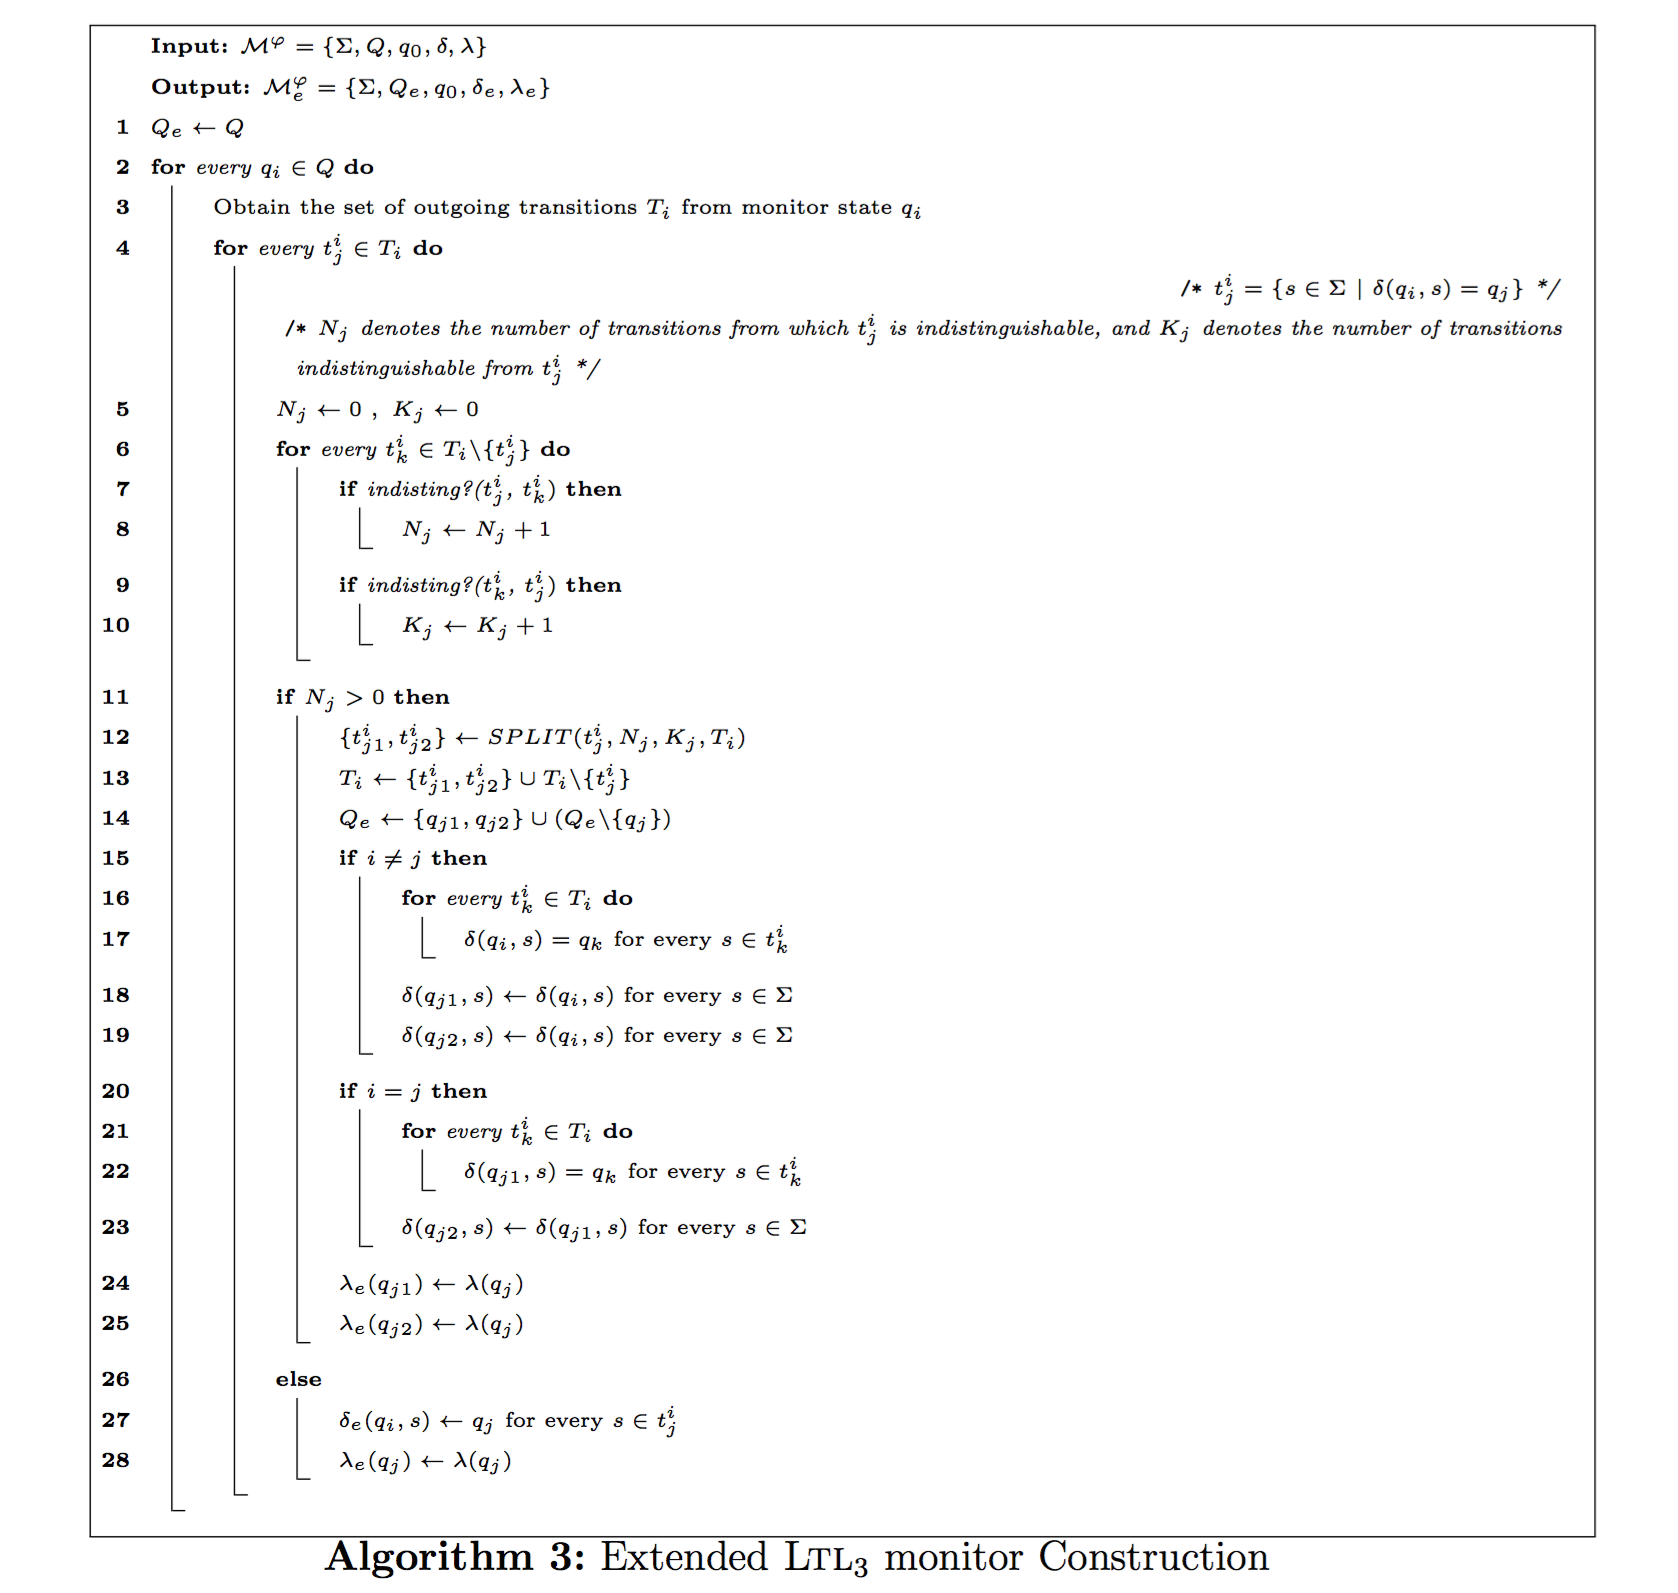
\includegraphics[scale=.25, angle=-360]{figures/ExltlMon}
 \end{figure}

 \end{frame}
 





\begin{frame}{Automata-based Synchronous Monitoring}


\begin{example}


Consider the \LTLtri monitor for $\varphi = \F (a \wedge b)$. 

%We have $\monitor^\varphi = \{ \{a, b\}, \{\monstate_0, \monstate_\top\}, \monstate_0, \delta, \lambda   \}$, where \\

\ \\

%$\delta(\monstate_0, \{a\}) = \delta(\monstate_0, \{b\}) = \delta(\monstate_0, \emptyset) = \monstate_0$  \\
%$\delta(\monstate_0, \{a, b\}) = \monstate_\top$. 




\iffalse
The set of outgoing 
transitions from monitor state $\monstate_0$ is $T_0 = \{t_0^0, t_\top^0\}$, 
where  $t_0^0 = \{\{a\}, \{b\}, \emptyset\}$ and $t_\top^0 = \{\{a,b\}\}$ are 
the outgoing transitions from monitor state $\monstate_0$ to monitor states 
$\monstate_0$ and $\monstate_\top$, respectively. We can verify that transition 
$t_0^0$ is \indist~from $t_\top^0$ since there is a state $\{a, b\} \in 
t_\top^0$ that is \covered~by transition $t_0^0$, i.e., $\dep (\{a, b\}, t_0^0) 
= \tru$. But $t_\top^0$ is not \indist~from $t_0^0$. Therefore, we have $N_0 = 
1$, $K_0 = 0$, $N_\top = 0$, and $K_\top = 0$. Since $N_0 > 0$, we \splt~$t_0^0$ 
into two transitions $t_{01}^0$ and $t_{02}^0$. Different \partitionn s of 
$t_0^0$ are as follows: 
\fi




\begin{figure}[H]
\centering

\begin{tikzpicture}[->,>=stealth',shorten >=1pt,auto,node distance=4.8cm,
                    semithick, initial text={}, initial where=right]
  \tikzstyle{every state}=[scale=0.65, every node/.style={scale=0.65}]

  \node[initial,state] (A)                {$\monstate_0$};
  \node[state, accepting]         (B) [left of  = A] {$\monstate_\top$};
 
  \path (A) edge              node {$ \{a,b\}$} (B)
     
            edge [loop above] node {$\{a\}, \{b\}, \emptyset$} (A) ;
  \path  (B) edge [loop above] node {$\tru$} (B);          
\end{tikzpicture}    
%\caption{$\monitor^\varphi$}
\end{figure}

The set of outgoing transitions from monitor state $q_0$ is $T_0 = \{t_0^0, t_\top^0\}$ where: 

\ \\ 

$t_0^0 = \{\{a\}, \{b\}, \emptyset\}$  \\
$t_\top^0 = \{\{a,b\}\}$

\ \\

We can verify that $t_0^0$ is indistinguishable from $t_\top^0$. Therefore we split transition $t_0^0$ into two transitions $t_{01}^0 = \{\{a\}\}$ and $t_{02}^0 = \{\{b\}, \emptyset\}$.


\end{example}

\end{frame}








\begin{frame}

\begin{example}


\begin{figure}[H]
\centering

\begin{tikzpicture}[->,>=stealth',shorten >=1pt,auto,node distance=4.8cm,
                    semithick, initial text={}, initial where=right]
  \tikzstyle{every state}=[scale=0.65, every node/.style={scale=0.65}]

  \node[state, visible on=<1->] (A)                {$\monstate_{01}$};
  \node[state, accepting, visible on=<1->]         (B) [left of  = A] {$\monstate_\top$};
  \node[state, visible on=<1->]         (D) [below of = B] {$\monstate_{02}$};

  \path (A) edge   [visible on=<1->]           node {$ \{a,b\}$} (B)
                 edge [loop above, visible on=<2->] node {$\{b\}, \emptyset$} (A)
                 edge      [bend left=20, visible on=<2->]     node   {$\{a\}$} (D)
        (B) edge [loop above, visible on=<1->] node {$\tru$} (B)
        (D) edge [visible on=<3->]                node {$\{a,b\}$} (B)
        (D) edge       [bend left=15, visible on=<3->]             node {$\{b\}, \emptyset$} (A)
        (D) edge [loop below, visible on=<3->] node {$\{a\}$} (D);

\end{tikzpicture}    
\end{figure}


Note that we have

\begin{center}
$\lambda(\monstate_{01}) = \lambda(\monstate_0) = ?$\\
$\lambda(\monstate_{02}) = \lambda(\monstate_0) = ?$
\end{center}


\end{example}

\end{frame}



\begin{frame}{Automata-based Synchronous Monitoring}

\begin{example}


Suppose $s=\{a,b\}$ is the current global state of the system and Let $\varphi = \F (a \wedge b)$. The initial state of the monitors is as follows:\\


\begin{center}

\begin{tabular}{| c |c |c |c|}
\multicolumn{3}{c}{sample} \\
\hline
&$a$&$b$&$\abstate_i^1$\\
\hline
$M_1$ & $\tru$  & $\natural$ & $\{\monstate_{02}, \monstate_\top\}$\\
$M_2$ & $\natural$ & $\tru$ &  $\{\monstate_{01}, \monstate_\top\}$\\
$M_3$ & $\natural$ & $\natural$ &  $\{\monstate_{01},\monstate_{02}, 
\monstate_\top\}$ \\
$M_4$ & $\natural$ & $\natural$ &  $\{\monstate_{01}, \monstate_{02}, 
\monstate_\top\}$\\
%$M_5$ & $\natural$ & $true$ \\
\hline
\end{tabular} 
\quad
\begin{tabular}{| c |c|}
\multicolumn{2}{c}{round 1} \\
\hline
&$\abstate_i^2$\\
\hline
$M_1$ & crashed\\
$M_2$ & $\{\monstate_\top\}$\\
$M_3$ & $\{\monstate_{01}, \monstate_\top\}$ \\
$M_4$ & $\{\monstate_{01}, \monstate_\top\}$ \\
%$M_5$ & $\natural$ & $true$ \\
\hline
\end{tabular}
\end{center}

\begin{center}

\begin{tabular}{| c |c|}
\multicolumn{2}{c}{round 2} \\
\hline
&$\abstate_i^3$\\
\hline
$M_1$ & crashed\\
$M_2$ & crashed\\
$M_3$ & $\{\monstate_\top\}$ \\
$M_4$ & $\{\monstate_{01}, \monstate_\top\}$ \\
%$M_5$ & $\natural$ & $true$ \\
\hline
\end{tabular} 
\quad
\begin{tabular}{| c |c|}
\multicolumn{2}{c}{round 3} \\
\hline
&$\abstate_i^4$\\
\hline
$M_1$ & crashed\\
$M_2$ & crashed\\
$M_3$ & $\{\monstate_\top\}$ \\
$M_4$ & $\{\monstate_\top\}$ \\
%$M_5$ & $\natural$ & $true$ \\
\hline
\end{tabular} 
\end{center}




\end{example}

\end{frame}




